\chapter{The High Granularity Calorimeter}
\label{chap:hgcal}

\section{The High Luminosity LHC}

Run~2 of the LHC is now complete, with over $\SI{150}{\fb}$ of data collected at $\sqrt{s}\,=\,\SI{13}{TeV}$. %original target was 150 Run 1 plus Run 2
This was achieved partly because the machine was eventually operated at twice its nominal instantaneous luminosity, resulting in values of at $\SI{2e34}{\lumi}$ during 2018.
The second long shutdown (LS2) commenced following the completion of Run~2 and will last until 2021.
During this time various improvements to the LHC will be made, including a substantial upgrade to the injection system.
The machine will also be readied for operation at $\SI{7}{TeV}$ per beam.
However these upgrades will not substantially affect the conditions experienced by the LHC experiments; 
the peak instantaneous luminosity is not envisaged to increase beyond $\SI{2e34}{\lumi}$.
As such no major changes are required to the CMS detector during LS2, although various improvements are planned: 
these include upgrades to the muon system and HCAL barrel.
Therefore the expectation for Run~3, commencing in 2021 with two years of high-avalaibility data-taking in 2022 and 2023, 
is that a further $\SI{150}{\fb}$ of data at will be accumulated. 
%See here for details of LS2 and Run 3: https://indico.cern.ch/event/773482/contributions/3213751/attachments/1763994/2863045/LHC-Run2.CMS.Dec18.JW.pdf

Beyond Run~3, the usefulness of running the LHC with its current parameters decreases.
In order to reduce the statistical error on physics measurements by a factor of two, high-availability operation for more than ten years would be required.
Therefore a major upgrade to the LHC is planned, referred to as the Phase~2 upgrade, to maximise its physics reach.
%insert info about what is actually being upgraded here? %TODO learn a bit about the things below 
%The technological innovations facilitating the upgrade include $\SI{12}{T}$ superconducting magnets, compact and precise superconducting cavities, and new beam collimation technology.
The resulting High~Luminosity~LHC (HL-LHC) \cite{HLLHC} will have an nominal levelled instantaneous luminosity of $\SI{5e34}{\lumi}$, 
permitting a total of $\SI{3000}{\fb}$ of data to be collected by the mid-2030s.
The current planned schedule of the future running of the LHC and HL-LHC is summarised in Figure~\ref{fig:hgcal_LHCschedule}.

The corresponding mean pileup is per bunch crossing is 140; however an additional 50\% beyond the nominal value is allowed for in the HL-LHC design, 
which would result in values of up to 200.
This consitutes a major change, and the environment will be significantly harsher than with the current LHC conditions, 
posing serious challenges to the detectors in terms of radiation tolerance and reconstruction in high pileup.
Therefore in order to maintain or improve upon the excellent performance exhibited in Run~2, a suite of upgrades to the CMS detector are planned.
One part of this upgrade will be the replacement of the current CMS endcap calorimeters with the high granulaity calorimeter (HGCAL).

%FIXME this figure is out of date
\begin{figure}[h!]
  \centering
  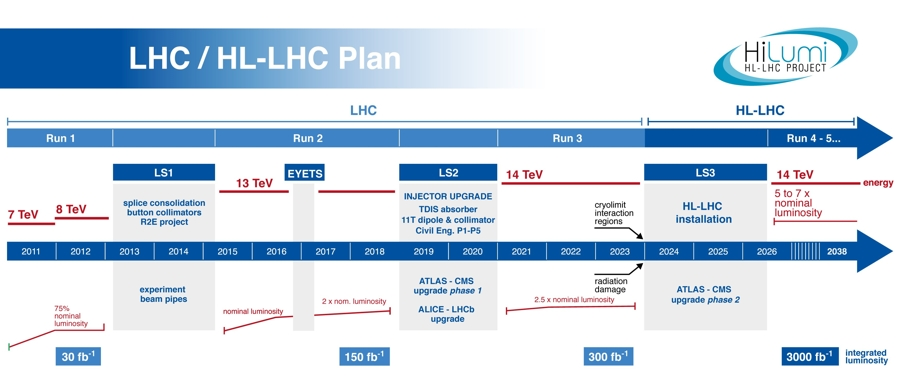
\includegraphics[width=\textwidth]{Figures/HGCAL/LHCschedule.jpg}
  \caption[Planned LHC and HL-LHC schedule]
  {The planned schedule for the operation of the LHC and its high-luminosity upgrade.}
  \label{fig:hgcal_LHCschedule}
\end{figure}


\section{The HGCAL}
\subsection{Requirements}
\subsection{Design}
\subsection{Reconstruction}
\subsection{Performance}
\subsection{Beam tests}
